% Created 2017-06-05 Mon 10:57
\documentclass[9pt,lineo]{elife}

\usepackage{amsmath}
\usepackage{amssymb}
\usepackage[version=4]{mhchem}
\usepackage{siunitx}


              \usepackage[utf8]{inputenc}
\sisetup{detect-all}
\setcounter{secnumdepth}{0}
\date{\today}
\title{}
\hypersetup{
 pdfauthor={},
 pdftitle={},
 pdfkeywords={},
 pdfsubject={},
 pdfcreator={Emacs 25.1.2 (Org mode 8.3.5)}, 
 pdflang={English}}
\begin{document}

\begin{figure}
\begin{fullwidth}
\centering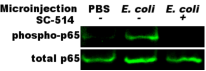
\includegraphics[width=0.5\linewidth]{./results/supplemental/p-65_western_blot.pdf}
\caption*{\textbf{Figure 4 - Supplement 2. }Western blot of phosphorylated p65 and total p65 in cell lysates from HIOs microinjected with PBS or live \textit{E. coli} and treated with IKK$\beta$ inhibitor SC-514 (1 $\mu$M) as indicated in the figure.}
\label{fig:fullwidth}
\end{fullwidth}
\end{figure}
\end{document}